\begin{figure}[!t]
\centering
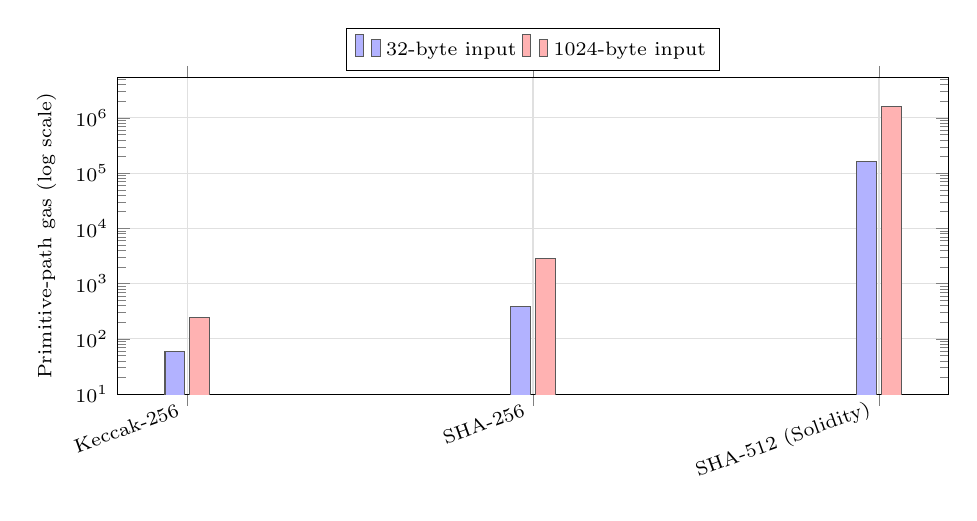
\begin{tikzpicture}
\begin{axis}[
  width=\columnwidth,
  height=5.6cm,
  ybar,
  bar width=7pt,
  ymode=log,
  log basis y=10,
  ymin=10,
  ylabel={Primitive-path gas (log scale)},
  symbolic x coords={Keccak-256,SHA-256,SHA-512 (Solidity)},
  xtick=data,
  x tick label style={rotate=20,anchor=east,font=\scriptsize},
  tick label style={font=\scriptsize},
  label style={font=\scriptsize},
  legend style={font=\scriptsize,at={(0.5,1.02)},anchor=south,legend columns=-1},
  grid=major,
  major grid style={black!12}
]
\addplot+[draw=black!65] coordinates {({Keccak-256},59) ({SHA-256},392) ({SHA-512 (Solidity)},162174)};
\addplot+[draw=black!65] coordinates {({Keccak-256},245) ({SHA-256},2879) ({SHA-512 (Solidity)},1614065)};
\legend{32-byte input,1024-byte input}
\end{axis}
\end{tikzpicture}
\caption{Local Hardhat EVM hash-primitive microbenchmark. Values are
\texttt{gasleft()} deltas around the isolated hash path under Solidity 0.8.20,
optimizer 200, \texttt{viaIR=true}, and the Paris EVM target. The SHA-512 bar
is a FIPS-vector-gated pure-Solidity reference, not the deployable evidence
path. It is not a public-testnet latency, fee, finality, or consensus result.}
\label{fig:hash-primitive-microbenchmark}
\end{figure}
